% ============================================================================
% Journal of Instrumentation (JINST) manuscript — skeleton v2 rewrite
% (2026-07-04, definitive-benchmark era; supersedes the 0.331-era draft).
%
% Build in the official JINST Overleaf template, which provides jinstpub.sty
% and JHEP.bst (https://www.overleaf.com/latex/templates/
%   jinst-journal-of-instrumentation-template/qkyhznbxvxkn).
% Drop this file + refs.bib + the figures/ directory into that project.
% Bibliography: BibTeX with JHEP.bst over refs.bib.
%
% EVERY number in this file is emitted by paper/make_paper_numbers.py
% (paper/numbers.json / numbers.md) from the committed benchmark artifacts,
% or carries an inline comment naming its artifact. Do not edit numbers by
% hand; regenerate them.
% ============================================================================
\documentclass[a4paper,11pt]{article}
\pdfoutput=1
\usepackage{jinstpub}

\usepackage{amsmath}
% jinstpub loads newtxmath, which already defines \Bbbk; neutralise it so
% amssymb can reload without a "command already defined" clash.
\let\Bbbk\relax
\usepackage{amssymb}
\usepackage{graphicx}
\usepackage{booktabs}
\usepackage{xcolor}
\usepackage{microtype}
\usepackage{orcidlink}
\usepackage{tikz}
\usetikzlibrary{shapes.geometric, arrows.meta, positioning, fit, backgrounds}
% JINST recommends line numbers on submission; harmless if lineno is absent.
\IfFileExists{lineno.sty}{\usepackage[mathlines]{lineno}\linenumbers}{}

% Title chosen by the authors (2026-07-05).
\title{Towards LLM-Powered Automation of a Dark Matter Constraint Repository}

\author[a,1]{Lanqing Yuan\,\orcidlink{0000-0003-0024-8017}}
\author[a]{and Karthik Ramanathan\,\orcidlink{0000-0003-4215-7834}}

\affiliation[a]{Department of Physics, Washington University in St.\ Louis,\\
  One Brookings Drive, St.\ Louis, MO 63130, U.S.A.}

\emailAdd{yuan.l@wustl.edu}
\note[1]{Corresponding author.}

\abstract{%
Community compilations of dark matter constraints are critical experimental
infrastructure, yet they are hand-curated by individual volunteers from
results that, in the ultralight dark matter literature, are still published
mostly as figures rather than as machine-readable records. We present an
LLM-agent pipeline that monitors arXiv, extracts exclusion limits from
papers through five competing channels (paper-provided source data,
tables, deterministic vector-path tracing, text, and plot vision), selects
among them with a validity-first policy, canonicalizes physics conventions
in a single vetted registry, and opens a pull request for expert review ---
nothing merges automatically. The large language model is confined to
perception and semantics; arithmetic, unit conversion, and candidate
selection are deterministic, testable code, and a set of pure-function
guards (including a text--vision corroboration gate) rejects
mis-extractions using only the model's own declared outputs. On a
328-paper benchmark of measured limits graded against the curator's own
repository, the production configuration reaches a median residual of
0.25~dex at a single LLM read per paper, with 15 of 258 compared papers
($\sim$6\%) beyond 3~dex. A confound-controlled two-arm comparison quantifies the model-tier
effect cleanly: swapping the frontier model for a small one costs
$+0.21$~dex in the paired median and roughly triples the catastrophic
tail. The dominant class of decade-scale errors was not visual
perception --- the vision channel's end-to-end median matches the text
channel's at $\sim$0.3~dex --- but unit and convention bookkeeping,
removed by contracts that forbid the model from converting units. We
report what helped, what did not (consensus voting bought $+0.003$~dex for
$3\times$ cost), and the measured run-to-run noise floor that bounds
single-run benchmark claims.}

\keywords{Analysis and statistical methods;
  Software architectures (event data models, frameworks and databases);
  Data processing methods}
% NOTE: confirm final keywords against the controlled JINST keyword list at
% submission; the three above are valid JINST keywords for an analysis/software paper.

\begin{document}
\maketitle

%=============================================================================
\section{Introduction}
\label{sec:intro}
%=============================================================================

The experimental search for ultralight dark matter is undergoing a
``renaissance''~\cite{snowmass_axion}, with new proposals targeting masses from
$10^{-22}$~eV to several eV~\cite{irastorza_review, kim_review}. The result is an
ever-denser landscape of constraints across at least 15 distinct \emph{coupling
types} (ways dark matter can interact with the Standard Model, e.g.\ axion--photon
or dark-photon kinetic mixing)~\cite{dp_cookbook}, each with its own units,
parameterisations, and confidence levels. Dark matter constraint repositories
compile these bounds into publication-quality \emph{exclusion plots}---the
mass--coupling regions ruled out---used across the field~\cite{axionlimits,
dp_cookbook, ohare_review}. The AxionLimits repository~\cite{axionlimits} tracks
over 600 limits and 160 projected sensitivities, yet is maintained by a single
volunteer who must find new results, digitise figures or tables, convert
parameterisations (e.g.\ $\chi$ vs.\ $g$~\cite{dp_cookbook}), write plotting code,
and regenerate figures. This is community-facing experimental infrastructure with
a single point of failure.

We treat this as an instrumentation and methods problem rather than an ``LLM
demo'': the questions that matter are reproducibility, quantified accuracy,
and auditable provenance. We present a pipeline that partially automates the
curation workflow: (1)~\textbf{discovery} via daily arXiv monitoring with
keyword filtering and LLM relevance classification; (2)~\textbf{extraction}
through five competing channels of differing semantic trust, with
deterministic guard rails and validity-first candidate selection;
(3)~\textbf{convention canonicalization} in a single vetted conversion
registry with fail-closed escalation; (4)~\textbf{integration} through
automated code generation with Abstract Syntax Tree (AST)-based insertion,
notebook updates, and plot regeneration; and (5)~\textbf{review} via pull
requests (PRs) with highlighted constraint plots---nothing merges without a
human expert. The system also includes a weekly preprint version checker and
a historical backfill workflow using
INSPIRE-HEP~\cite{inspirehep}.\footnote{Code, evaluation benchmark, and
prompts: \url{https://github.com/FaroutYLq/AutoAxionLimits}}

\paragraph{Contributions.}
To our knowledge, no existing system automates the full loop from discovery
through extraction, code integration, and human review for a live scientific
repository.
(i)~A multi-channel extraction architecture with validity-first candidate
selection and deterministic guard rails (section~\ref{sec:arch}).
(ii)~A convention-canonicalization system---truthful-declaration and
plotted-values contracts, a single-owner vetted conversion registry, and
fail-closed escalation to human review (section~\ref{sec:conv}).
(iii)~A 328-paper measured-limits benchmark against curator ground truth, with
confound-controlled methodology and a measured run-to-run noise floor
(section~\ref{sec:eval}).
(iv)~Quantified design lessons---what helped and what did not, including
consensus-voting and model-tier economics (section~\ref{sec:discussion}).
(v)~An open-source, human-in-the-loop deployment on the live literature
(sections~\ref{sec:integration} and~\ref{sec:cases}).

%=============================================================================
\section{Related work}
\label{sec:related}
%=============================================================================

\paragraph{LLM extraction from scientific documents.}
A growing body of work uses large language models to convert unstructured
scientific text into structured records. Dagdelen et al.~\cite{dagdelen2024structured}
fine-tune LLMs for joint entity and relation extraction from chemistry text, while
subsequent surveys and systems target materials-science data at
scale~\cite{schilling2024texttoinsight}, including table-focused extractors such as
MaTableGPT~\cite{yi2024matablegpt}. A complementary thread tackles the figure
modality directly: classical tools like WebPlotDigitizer~\cite{rohatgi2024wpd}
digitise plots with computer-vision-assisted manual input, and recent
vision--language methods such as DePlot~\cite{liu2023deplot} translate chart images
into tables for downstream reasoning. The closest precedent for automated
literature-to-database curation is the ChemDataExtractor lineage of
auto-generated materials databases~\cite{huang2020battery}, and the nearest
contemporaneous HEP system is a retrieval-augmented multi-agent framework
for interpreting searches beyond the Standard Model~\cite{cakir2026limits},
which operates on already-structured HEPData records. Our pipeline
differs in combining text, table, vision, and deterministic-geometry
modalities as \emph{competing channels} under deterministic selection and
guards, and in grounding the output in an executable scientific repository
rather than a structured record store or free-text knowledge base.

\paragraph{AI for science and literature infrastructure.}
Beyond extraction, agentic LLM systems now plan and execute research, from
autonomous chemistry~\cite{boiko2023autonomous} to end-to-end paper
generation~\cite{lu2024aiscientist}, building on science-specific foundation
models~\cite{taylor2022galactica}. In parallel, scholarly knowledge-base
efforts---literature graphs and open corpora~\cite{ammar2018literaturegraph,
lo2020s2orc}---automate monitoring and curation of the literature itself, and
machine learning is already pervasive in particle-physics
analysis~\cite{feickert2021livingreview}. Unlike these systems, which produce
hypotheses, prose, or static datasets, our work closes a narrower but fully
operational loop---discovery, extraction, code integration, and human-reviewed pull
requests---against a live, community-facing constraint repository, where every
automated output must survive a domain expert's review before acceptance.

%=============================================================================
\section{System architecture}
\label{sec:arch}
%=============================================================================

\begin{figure}[t]
\centering
\resizebox{\textwidth}{!}{%
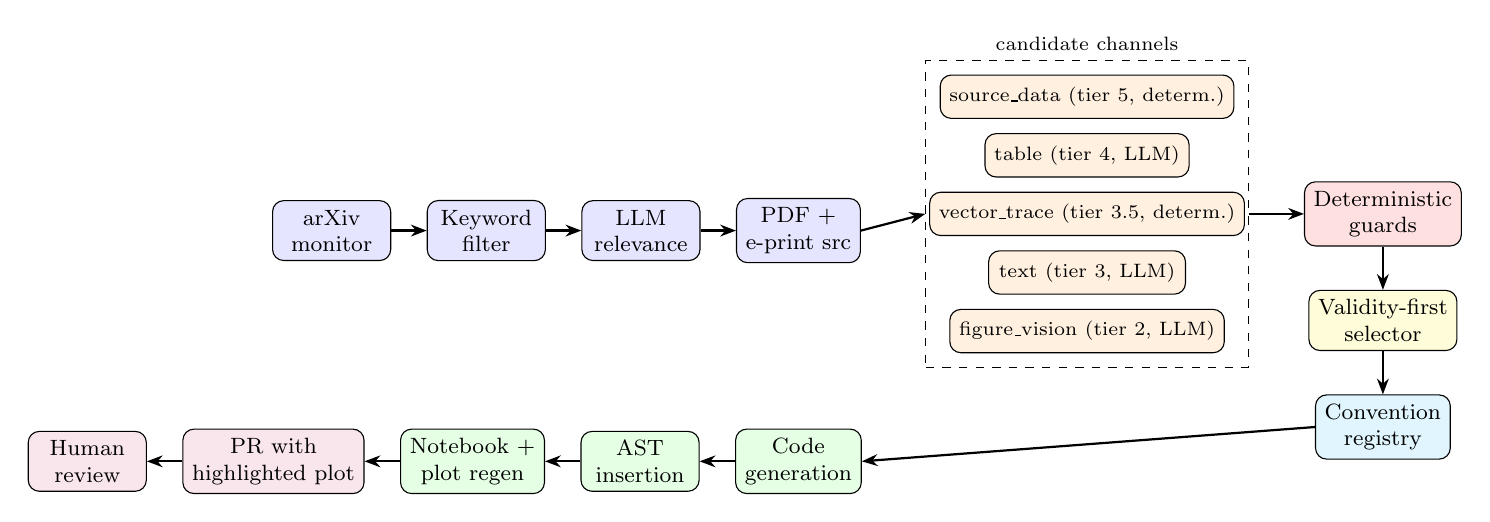
\begin{tikzpicture}[
    node distance=0.55cm and 0.45cm,
    block/.style={rectangle, draw, rounded corners, minimum height=0.7cm, minimum width=1.5cm, align=center, font=\footnotesize},
    chan/.style={rectangle, draw, rounded corners, minimum height=0.55cm, minimum width=2.5cm, align=center, font=\scriptsize},
    arrow/.style={-{Stealth[length=2mm]}, thick},
    lbl/.style={font=\scriptsize, text=gray},
]
% discovery row
\node[block, fill=blue!10] (arxiv) {arXiv\\monitor};
\node[block, fill=blue!10, right=of arxiv] (kw) {Keyword\\filter};
\node[block, fill=blue!10, right=of kw] (llm1) {LLM\\relevance};
\node[block, fill=blue!10, right=of llm1] (pdf) {PDF +\\e-print src};
% channel stack
\node[chan, fill=orange!12, right=1.0cm of pdf, yshift=1.7cm] (csrc) {source\_data (tier 5, determ.)};
\node[chan, fill=orange!12, below=0.18cm of csrc] (ctab) {table (tier 4, LLM)};
\node[chan, fill=orange!12, below=0.18cm of ctab] (cvec) {vector\_trace (tier 3.5, determ.)};
\node[chan, fill=orange!12, below=0.18cm of cvec] (ctxt) {text (tier 3, LLM)};
\node[chan, fill=orange!12, below=0.18cm of ctxt] (cvis) {figure\_vision (tier 2, LLM)};
\node[draw, dashed, inner sep=5pt, fit=(csrc)(cvis), label={[font=\scriptsize]above:candidate channels}] (chanbox) {};
% guards + selection + conventions
\node[block, fill=red!12, right=0.7cm of chanbox] (guards) {Deterministic\\guards};
\node[block, fill=yellow!15, below=of guards] (select) {Validity-first\\selector};
\node[block, fill=cyan!12, below=of select] (conv) {Convention\\registry};
% integration row (right to left, below)
\node[block, fill=green!10, below=2.1cm of pdf] (codegen) {Code\\generation};
\node[block, fill=green!10, left=of codegen] (ast) {AST\\insertion};
\node[block, fill=green!10, left=of ast] (notebook) {Notebook +\\plot regen};
\node[block, fill=purple!10, left=of notebook] (pr) {PR with\\highlighted plot};
\node[block, fill=purple!10, left=of pr] (human) {Human\\review};
\draw[arrow] (arxiv) -- (kw);
\draw[arrow] (kw) -- (llm1);
\draw[arrow] (llm1) -- (pdf);
\draw[arrow] (pdf.east) -- (chanbox.west);
\draw[arrow] (chanbox.east) -- (guards.west);
\draw[arrow] (guards) -- (select);
\draw[arrow] (select) -- (conv);
\draw[arrow] (conv.west) -- (codegen.east);
\draw[arrow] (codegen) -- (ast);
\draw[arrow] (ast) -- (notebook);
\draw[arrow] (notebook) -- (pr);
\draw[arrow] (pr) -- (human);
\end{tikzpicture}
}
\caption{Pipeline architecture. Papers flow from arXiv through keyword and LLM
filtering into five competing extraction channels of differing semantic trust.
Deterministic guards (pure functions over the model's declared outputs) reject or
demote candidates; a validity-first selector picks the winner; the convention
registry maps it to the repository's canonical variable or fails closed to human
review. Integration produces a pull request with a highlighted constraint plot;
nothing merges without a human expert.}
\label{fig:architecture}
\end{figure}

Figure~\ref{fig:architecture} shows the end-to-end pipeline. Its design
principle, arrived at empirically (section~\ref{sec:discussion}), is to keep
the LLM confined to \emph{perception and semantics}---reading text, tables,
axes, and curves, and declaring what it read---while arithmetic, unit
conversion, and candidate selection are deterministic, testable code.

\subsection{Discovery and triage}
A daily job pulls new submissions from the arXiv feed and narrows them in three
steps of increasing cost: a cheap keyword filter against a curated set of experiment
names and coupling jargon; a short LLM relevance call on title and abstract that
decides whether the paper actually reports a new exclusion limit (as opposed to a
theory paper, a recast, or an unrelated result); and a download of the survivors'
PDF and e-print source. Two sibling workflows reuse the same machinery: a weekly
preprint checker that re-extracts tracked papers when a new arXiv version
appears---it once caught a JWST dark-photon search~\cite{jwst_dp} that demoted a
measured limit to a projection on publication---and a historical backfill that
mines INSPIRE-HEP~\cite{inspirehep} for older high-citation papers. Pipeline state
(processed papers, known preprint versions) is persisted in git alongside the code.

\subsection{Multi-channel extraction}
\label{sec:channels}
Extraction turns a paper into a structured record: coupling type, a list of
$(\text{mass}, \text{coupling})$ data points, the declared units/convention,
whether the result is a new limit or a projection, an extraction-confidence
score, and notes. Rather than one extraction path, the agent produces
\emph{candidates} through up to five channels of differing semantic trust
(table~\ref{tab:channels}), staged as: a cheap pre-classification pass; a
stage-1 text/table read of the parsed PDF (PyMuPDF~\cite{pymupdf}); a cheap
stage-2a pass that identifies the relevant figure and reads its axis labels
and ranges; and a stage-2 vision trace of the rendered figure pages. Two
channels are deterministic: \texttt{source\_data} harvests numeric files
shipped in the paper's own e-print source (pgfplots \texttt{.dat} tables,
ancillary files)---exact where present---and \texttt{vector\_trace} extracts
curve geometry directly from the vector paths of PDF figures, with a single
cheap LLM call used only to identify \emph{which} path is the limit curve.
Prompt-injection defences strip control characters and wrap the paper text in
sentinel delimiters so that instructions embedded in a PDF cannot hijack the
model.

\begin{table}[t]
\caption{Candidate extraction channels and their semantic trust tiers. Tier
enters the validity-first selector (section~\ref{sec:select}) only after all
validity criteria; higher tier wins among equally valid candidates.}
\label{tab:channels}
\centering
\small
\begin{tabular}{@{}lcl@{}}
\toprule
\textbf{Channel} & \textbf{Tier} & \textbf{Nature} \\
\midrule
\texttt{source\_data}  & 5   & deterministic numeric files from the paper's own e-print source \\
\texttt{table}         & 4   & LLM read of a tabulated bound \\
\texttt{vector\_trace} & 3.5 & deterministic vector-path geometry; curve identity by one cheap LLM call \\
\texttt{text}          & 3   & LLM read of bounds stated in prose \\
\texttt{figure\_vision}& 2   & LLM trace of the rendered exclusion plot \\
\bottomrule
\end{tabular}
\end{table}

\subsection{Validity-first candidate selection}
\label{sec:select}
Candidates are ranked by a lexicographic quality tuple in which every
\emph{validity} criterion outranks every \emph{preference} criterion, and raw
point count comes last: values in physically allowed ranges $\rightarrow$
non-degenerate curve $\rightarrow$ recoverable under a clean power-of-ten
correction $\rightarrow$ convention known to the registry $\rightarrow$
channel tier $\rightarrow$ corroborated by an independent channel
$\rightarrow$ self-reported confidence $\rightarrow$ point count. A sparse
text bound of a few points (e.g.\ a headline number quoted in prose) is
demoted below a traceable multi-point curve \emph{unless} it is corroborated,
so a single quoted number cannot override an actual digitised constraint, yet
a corroborated point limit can still beat an uncorroborated trace. Candidates
whose declared convention failed convention review are demoted rather than
silently converted. This encodes a hard-won lesson: ``more points'' is not
``more trustworthy,'' and neither is ``more confident.''

\subsection{Deterministic guards}
\label{sec:guards}
A set of guards rejects or demotes candidates \emph{before} selection. All are
pure functions over the model's own declared outputs---no additional API
calls---which makes them fully unit-testable and free to run everywhere.
Wrong-curve gates use the model's own notes (a note admitting ``traced the
projection, not the limit'' rejects the candidate), the abstract-stated mass
window (a curve outside the window the paper itself announces is demoted), and
regime checks. The \textbf{text--vision corroboration gate} rejects a vision
trace that deviates by more than 2~dex from an in-range text anchor over their
shared mass support---an independent cross-check between channels that fired
19 times in the production-configuration benchmark run
(section~\ref{sec:results}). Range validation applies snap-to-decade
suppression when the declared convention is non-canonical, so a legitimate
squared-coupling axis is not ``corrected'' into a wrong decade.

\subsection{Convention canonicalization}
\label{sec:conv}
This is the layer that most distinguishes a working pipeline from a naive one,
and it is pure physics, not perception. The same bound is published in
incompatible $y$-variables across papers---$g$, $g^2$, $g^2/4\pi$, $1/f_a$,
$\Lambda$, $\varepsilon^2$, decay rates, lifetimes---and even across files
within one coupling type, with the conversion often living in the repository's
plotting code rather than in the paper. Cross-convention comparison creates
multi-decade \emph{apparent} errors that are not extraction errors. Three
rules govern the layer:

\textbf{Truthful declaration.} Every channel declares the convention of the
values it \emph{emits}. \textbf{Plotted values.} The vision channel never
converts: it emits raw axis values and declares the plotted quantity, and an
axis read-back (a measurement) overrides a canonical-claiming declaration (an
assertion). Asking the model to convert units invites double conversion (the
model converts \emph{and} the registry converts again) or zero conversion;
both produced $\sim$8~dex errors on correct readings before these contracts
were adopted (section~\ref{sec:anatomy}). \textbf{Single-owner conversions.}
A vetted registry is the only place conversions happen. Its factors were not
guessed or prompted out of a model: they were derived with the agentic physics
assistant Get Physics Done (GPD)~\cite{gpd}, code-verified against the
repository plotting source, and citation-audited against the underlying
literature (the Damour--Donoghue dilaton parameterisation; the axion
derivative-coupling on-shell reduction giving the $2m_N$ factor).
Table~\ref{tab:conventions} lists the families.

\begin{table}[t]
\caption{Per-file convention conversions applied to both extracted and reference
curves before scoring (implemented in \texttt{evaluation/conventions.py}). The
factors were derived with GPD~\cite{gpd}, code-verified against the repository
plotting source, and citation-audited against the literature. $m_n=0.93957$,
$m_p=0.93828$~GeV.}
\label{tab:conventions}
\centering
\small
\begin{tabular}{@{}p{3.0cm}p{3.3cm}p{2.6cm}p{3.6cm}@{}}
\toprule
\textbf{Coupling family} & \textbf{Repository canonical} & \textbf{Common paper variable} & \textbf{Conversion to canonical} \\
\midrule
AxionNeutron / AxionProton & dimensionless $g_{aN}$ & GeV$^{-1}$ derivative $g_{aNN}=C_N/2f_a$ & $g_{aN}=2m_N\,g_{aNN}$ \\
AxionNeutron (SNO file only) & dimensionless $g_{an}$ & $g_{an}/m_n$ [GeV$^{-1}$] & $g_{an}=m_n\cdot(\text{stored})$ (per-file) \\
Scalar / dilaton & dimensionless $d_e$, $d_{m_e}$ & fifth-force strength $\alpha$ & $d=Q^{-1}\sqrt{\alpha}$, $Q^{-1}=500$ (photon/nucleon), $4000$ (electron) \\
DarkPhoton & kinetic mixing $\chi=\varepsilon$ & $\varepsilon^2$ & $\chi=\sqrt{\varepsilon^2}$ \\
AxionEDM & $g_{an\gamma}$ ($=g_d$) [GeV$^{-2}$] & $1/f_a$ [GeV$^{-1}$] & $g_{an\gamma}=3.7\times10^{-3}\,(1/f_a)$ \\
AxionMass & normalized $1/f_a$-based coupling & $f_a$ [GeV] & per-point reciprocal $f_a \to 1/f_a$ \\
\bottomrule
\end{tabular}
\end{table}

Two further traps the layer handles: \emph{sentinel values}---rows valued
$10^{20}$, $10^{30}$, $10^{99}$ are not data but the closing vertices of a filled
polygon, and are stripped (floor $10^{19}$); and \emph{header-vs-value
disagreement}---some scalar files carry a header claiming $d_e$ while the magnitudes
are inconsistent with it, so classification uses the value range, not the header
string. The comparator maps both the extracted curve and the reference curve to the
canonical variable \emph{before} any residual is computed.

Everything outside the vetted vocabulary \textbf{fails closed}. A
\emph{foreign-quantity screen} catches declarations naming physics outside a
coupling's vetted vocabulary (e.g.\ a decay-width axis on a coupling plot):
matching is against the vetted vocabulary itself, never by substring heuristics
on free text, which we found silently suppress review flags. Unconvertible
candidates surface as a \texttt{[CONVENTION REVIEW]} flag with capped confidence
at runtime---routed to a human---and are excluded as convention gaps on the
evaluation side rather than scored raw; ``converted from \dots'' declarations
are never re-converted. Getting these factors exactly right is a small but
exacting derivation task, and treating it as such---rather than as a prompting
problem---is what made the registry trustworthy enough to apply automatically.

\subsection{Integration and review}
\label{sec:integration}
The selected, canonicalized result is turned into a code change. The LLM generates
a \texttt{@staticmethod} for the relevant plotting class (a post-generation guard
re-inserts the decorator if the model omits it); the method is inserted using Python's
AST module, locating the last method in the target class---never by regex
string-matching, which could corrupt the file. A notebook cell calling the new method
is inserted via \texttt{nbformat} and the figure is regenerated headlessly via
\texttt{nbconvert}; when the new limit's mass range falls outside the figure's
conventional axis window, the axis is automatically widened (never shrunk) so the
limit is plotted rather than silently dropped off the plot edge. Every change becomes
a pull request, never an automatic merge. Confidence tiers in the PR title
(\texttt{[LOW CONFIDENCE]}, \texttt{[NEEDS REVIEW]}, \texttt{[CONVENTION REVIEW]})
route reviewer attention. The key reviewer aid is a \emph{highlighted plot}:
the full constraint figure rendered with all existing limits greyed out and
only the new proposed curve in red, so a domain expert can sanity-check the
proposal visually in seconds without reading code
(figure~\ref{fig:showcase} in the case study of section~\ref{sec:cases}).

\subsection{Robustness and operations}
\label{sec:ops}
Three operational defences matter in practice. \emph{Availability fail-fast:}
billing and authentication errors abort the entire run without marking the
current paper processed or failed---an availability error is a property of the
run, not the paper; failing ``closed'' to a default answer would silently
convert an outage into wrong science. \emph{Runtime configuration assertion:}
the extraction driver asserts the resolved model identity at startup rather
than trusting environment configuration---a lesson from an incident in which a
silently substituted model confounded a benchmark
(section~\ref{sec:confound}). \emph{Cost containment:} prompt caching saves
20--36\% of token spend (measured across production runs), and all model calls
retry with exponential backoff on rate-limit errors. At production volume
(1--3 papers/day) the per-paper cost is cents to $\sim$a dollar depending on
whether the vision channel runs; this is far below the expert time it
substitutes for.

%=============================================================================
\section{Evaluation methodology}
\label{sec:eval}
%=============================================================================

\subsection{Ground truth}
\label{sec:gt}
We evaluate on 328 papers spanning the repository's coupling types, chosen as
curated repository data files~\cite{axionlimits} that carry a known arXiv ID
(the full registry holds 434 file entries over 347 distinct arXiv IDs, one of
which entered after the benchmark pool froze). The benchmark scope is
\textbf{measured limits only}: the 25 entries (18 papers) that record
\emph{projected} sensitivities are excluded, because projections are of less
interest to the community than measured bounds, and because they typically
embed detector-scenario assumptions --- a single figure often shows several
curves for different assumed configurations --- which makes a single
ground-truth curve ill-defined and hard to record faithfully. (The production
pipeline still processes projection papers; their proposals are simply
labelled \texttt{[PROJECTION]} and stored separately.) The ground truth (GT) for each paper is the
upstream repository's own digitised curve---\emph{never} a curve digitised by
our own model, which would be circular. This choice carries a consequence: the
reference was itself digitised and rescaled from the same paper, so a perfect
extraction still shows a nonzero residual equal to the upstream digitisation
gap, measured independently at $\sim$0.034~dex on re-digitised table/text
sources ($N=10$; the figure-only component of this yardstick remains
unmeasured)---far below the residuals we report, so what we report is
extractor error, not yardstick artefact. Eighteen GT entries (16 papers, 15
of them in the benchmark pool) carry documented, reversible exclusions, used
only when the GT itself can grade no extraction (prediction-band files,
published-only data)---never because the extractor fails a paper. Each
entry declares its unit conversions in a header, applied at ingestion.

\subsection{Metrics}
\label{sec:metrics}
We compare in $\log_{10}$--$\log_{10}$ space. A log--log interpolation of the
extracted points is evaluated at each GT mass $m_i$ inside the extracted mass
range, giving a per-point residual
\begin{equation}
  r_i = \bigl|\log_{10} g_{\rm ext}(m_i) - \log_{10} g_{\rm truth}(m_i)\bigr|
  \label{eq:residual}
\end{equation}
where $0.3~\text{dex} \approx$ a factor of two. A paper's residual is
the median $r_i$, and a reverse pass (interpolating GT onto extracted masses)
flags curves that run past the true range. We report the \emph{micro-median}
(the median over papers) and a \emph{macro average} (the \emph{mean} of
per-coupling-type medians, equal weight per type)---the latter is the
tail-sensitive statistic, since it cannot be bought by accuracy on the most
common coupling type, and as a mean it is deliberately sensitive to a single
badly-failing type. ``Compared'' papers are those scored against a
same-coupling GT curve with finite residual; a paper is \emph{catastrophic}
if its residual exceeds 3~dex. Convention-gap papers are excluded, not
scored raw: scoring a units mismatch as extraction error is the larger sin,
and the exclusion is reported. Every benchmark statistic in
section~\ref{sec:results} is emitted by a committed script
(\texttt{paper/make\_paper\_numbers.py}) from the committed benchmark
artifacts, with each definition pinned in code, so a referee can reproduce
those values from the public repository; numbers drawn from supporting
studies (the vote probe, the channel surveys, the error-anatomy case) cite
their specific artifacts inline where they appear.
Table~\ref{tab:disposition} gives the disposition of all 328 papers in the
production-configuration arm.

\begin{table}[t]
\caption{Disposition of the 328 benchmark papers (production-configuration arm,
measured-limits scope). Only ``compared'' papers with finite residual (258 of
262) enter the residual statistics.}
\label{tab:disposition}
\centering
\small
\begin{tabular}{@{}lcp{8.2cm}@{}}
\toprule
\textbf{Disposition} & \textbf{N} & \textbf{Meaning} \\
\midrule
compared             & 262 & scored against a same-coupling GT curve (4 with zero mass overlap) \\
no\_comparable\_gt   & 23  & predicted coupling has no GT curve in the pool (usually a misclassification) \\
convention\_mismatch & 19  & same coupling, unvetted parameterisation (a units gap, not extraction error) \\
excluded\_gt         & 15  & documented GT-side exclusion (section~\ref{sec:gt}) \\
no\_extracted\_points& 7   & pipeline returned a type but no data points \\
no\_prediction       & 1   & pipeline returned no coupling type \\
gt\_unusable         & 1   & GT curve has $<2$ usable points after sentinel stripping \\
\bottomrule
\end{tabular}
\end{table}

\subsection{Confound control}
\label{sec:confound}
We report our evaluation methodology's failure as a contribution, because the
repair generalises. During development, a full-pool comparison silently changed
the extraction \emph{model} and the pipeline \emph{code} together: a workflow
change had repointed the model environment variable, and the resulting
``regression'' (a $\sim$0.6~dex headline) was initially read as a code effect.
The comparison was retracted and replaced with an isolation design: (i) a
same-code A/B in which only the model differs, and (ii) a fixed-model A/B in
which only the code differs. (An earlier public preprint of this
work~\cite{autoaxion_preprint} reports pre-repair numbers under the old
consensus-voting architecture and is superseded by this manuscript.) The definitive benchmark
(section~\ref{sec:results}) runs both models on identical code, an identical
paper pool, identical transport, and identical vote count, with every
extraction fresh (no snapshot reuse), enabling a \emph{paired} per-paper
model comparison. Two further methodology measurements bound all claims:

\textbf{Noise floor.} Repeat runs of the same configuration leave the
aggregate median stable to within a 95\% bootstrap confidence interval of
$\pm0.06$~dex (Opus, $N{=}1$), measured by re-running extraction on a random
57-paper subset in matched configuration---same code, transport, and vote
count---and pairing each fresh read with its benchmark counterpart, so that
``repeat~1'' is the definitive run itself and ``repeat~2'' a fresh matched
re-run (\texttt{evaluation/eval\_runs/noise\_floor\_100\_reuse/}). The floor
is dominated by channel-routing flips: 19\% of papers route to a different
channel (text $\leftrightarrow$ vision) between runs, populating a heavy
per-paper tail ($|\Delta|$ up to $\sim$6~dex) atop a stable core in which most
papers reproduce to $<$0.03~dex (median run-to-run difference $|\Delta|=0.03$~dex;
Fig.~\ref{fig:noisefloor}). Single-run deltas below the aggregate floor are
not signal; we report first decimals, not third. \textbf{Vote-count probe.} The
same transport-matched 30-paper probe measured $N=3$ consensus voting
against single reads ($N=1$) on the production model, isolating the vote
count from all other variables (section~\ref{sec:votes}).

\begin{figure}[t]
\centering
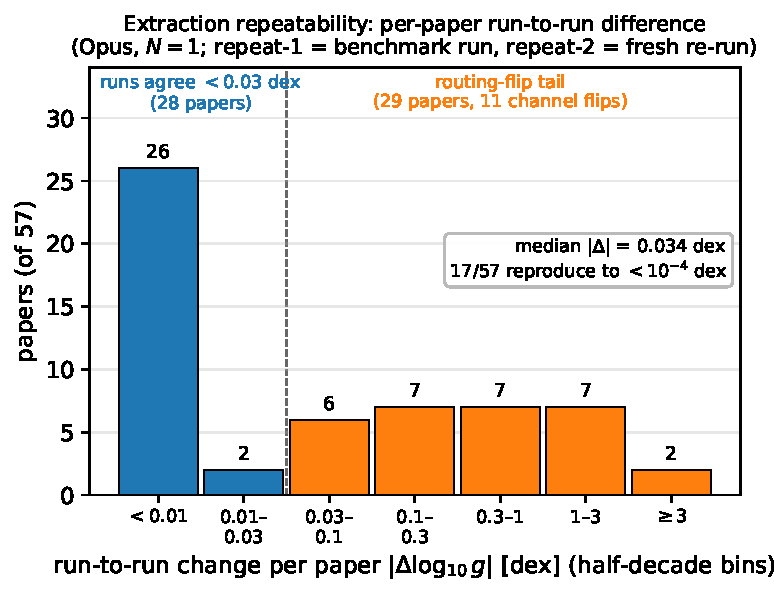
\includegraphics[width=0.72\textwidth]{figures/noise_floor_hist.pdf}
\caption{\textbf{Extraction repeatability.} Per-paper run-to-run change in the
median coupling residual, $|\Delta\log_{10} g|$, between the definitive Opus run
(``repeat~1'') and a fresh matched-configuration $N{=}1$ re-read (``repeat~2'')
of a random 57-paper subset. Bins are half-decade (log-spaced) because $|\Delta|$
spans four orders of magnitude; the leftmost bin absorbs the reproducible core
(17 of 57 papers agree to $<10^{-4}$~dex). The distribution is bimodal: a stable
core (blue; 28 papers reproduce to $<$0.03~dex) and a heavy routing-flip tail
(orange; 29 papers, of which 11 route to a different extraction channel between
runs). Despite this tail the \emph{aggregate} median moves by only
$\pm0.06$~dex (95\% bootstrap CI), because the tail papers are a minority and the
pool median is robust; the per-paper standard deviation at $n{=}2$ is
$|\Delta|/\sqrt{2}$.}
\label{fig:noisefloor}
\end{figure}

%=============================================================================
\section{Results}
\label{sec:results}
%=============================================================================

All numbers in this section are generated by
\texttt{paper/make\_paper\_numbers.py} from the committed artifacts of the
definitive benchmark run (both arms on the fixed pipeline, $N=1$;
measured-limits scope, \texttt{evaluation/eval\_runs/final2\_*/metrics\_noproj.json}).

\subsection{Headline: the definitive two-arm benchmark}
\label{sec:headline}
Table~\ref{tab:results} shows both arms: the production configuration
(Claude Opus~4.8~\cite{anthropic_claude}) and the same pipeline on a small
model (Claude Haiku~4.5). The production arm reaches a \textbf{0.2509~dex}
micro-median over 258 compared papers, at a single LLM read per paper. The
same denominator caveat applies to both arms: 258 of 328 processed papers
yield a comparable finite residual, and the remainder
(table~\ref{tab:disposition}) --- misclassifications, empty extractions, and
excluded convention gaps --- do not enter the median, so the headline
describes accuracy \emph{given} a comparable extraction, not end-to-end
success on every paper. The deterministic guards are
load-bearing at this scale, not theoretical: the text--vision corroboration
gate rejected 19 vision candidates and the convention layer flagged 20 papers
for human review in this single benchmark run (the scoring-side
\texttt{convention\_mismatch} disposition of table~\ref{tab:disposition} is a
related but distinct count: runtime flags mark the extraction, the
disposition marks the GT comparison). Coupling-type classification
is 92.3\% accurate ($N=313$ graded against the repository's directory
structure); the auxiliary labels reach 100\% (\emph{is new limit}) and
100\% (\emph{is projection}) against an independent LLM labeler ($N=30$;
a 15-paper human audit of that labeler found 15/15, 15/15, and 14/15
agreement on the three labels) --- notably, all the label errors of the
full-scope benchmark sat on projection papers.

\begin{table}[t]
\caption{The definitive two-arm benchmark: both models on the identical fixed
pipeline, identical 328 measured-limit papers, $N=1$, identical transport. ``Compared'' =
scored against a same-coupling GT curve with finite residual. Catastrophic =
residual $>3$~dex.}
\label{tab:results}
\centering
\small
\begin{tabular}{@{}lcc@{}}
\toprule
 & \textbf{Opus 4.8 (production)} & \textbf{Haiku 4.5} \\
\midrule
micro-median residual   & \textbf{0.2509 dex} & 0.6474 dex \\
macro average (mean of per-type medians) & \textbf{0.629 dex}  & 3.259 dex \\
papers compared         & 258 & 225 \\
catastrophic ($>3$ dex) & 15 ($5.8\%$ of compared) & 41 ($18.2\%$) \\
$>1$ dex                & 49 & 91 \\
mean fraction of points within 0.3 dex & 53.4\% & 30.8\% \\
mean mass-range coverage & 85.6\% & 77.4\% \\
\bottomrule
\end{tabular}
\end{table}

\subsection{Code effect at fixed model}
\label{sec:codeeffect}
The pre-rework baseline---the same production model on the \emph{old} code
with $N=3$ consensus voting, rescored on the same measured-limits
scope---scored 0.2333~dex micro / 1.462~dex macro. The
fixed pipeline at $N=1$ lands at 0.2509 / 0.629: headline parity within the
measured noise floor at \textbf{one-third the LLM reads per paper}. The
macro average moved from 1.462 to 0.629~dex, but we do not claim that
improvement as robust: being a mean over types with per-type medians, it is
dominated by single-paper coupling types, and most of the delta traces to
one such type flipping from a catastrophic to a clean extraction; no
macro-level noise floor has been measured. Parity itself is conservative,
not flattering: the hardened registry now excludes as convention gaps papers
the old scoring compared raw, so the fixed pipeline is graded on a stricter
contract. A 77-paper paired code A/B at fixed model supports the same
conclusion ($-0.016$~dex, $+4$ papers coverage;
\texttt{evaluation/eval\_runs/final\_full346\_haiku\_report.md}).

\subsection{Model effect, measured cleanly}
\label{sec:modeleffect}
Pairing the 212 papers compared in \emph{both} arms---identical code, papers,
transport, and scorer; only the model differs---gives the clean model-tier
measurement: \textbf{Haiku $-$ Opus $= +0.210$~dex median}, with the frontier
model better on 135 papers, the small model on 37, and 40 within
$\pm$0.05~dex. An earlier estimate on a 77-paper shared subset
(\texttt{evaluation/eval\_runs/haiku\_regression\_causal\_digest.md}) had put
the gap at $+0.95$~dex; the shrinkage decomposes into failure-tail sampling
(the subset over-sampled hard vision papers) and a code amplifier: the pre-fix
plane bookkeeping (section~\ref{sec:anatomy}) turned the small model's
erratic convention declarations into decade-scale errors, so a code bug was
being charged to the model. Fixing the code moved the small model's own
operating point from 0.975 to 0.66~dex (full-scope values). The retraction cuts one way only:
the tail and coverage gaps are real and large---41 vs 15 catastrophic papers,
macro average 3.259 vs 0.629~dex, 225 vs 258 compared (papers the small model
fails to extract never enter its residual median, so the arm-level headline
\emph{understates} the gap). The correct summary: a modest median gap, a
large tail gap.

\subsection{Vote-count economics}
\label{sec:votes}
The transport-matched probe (30 papers, stratified toward the
vision/ambiguous tail where voting should matter most;
\texttt{evaluation/eval\_runs/nprobe\_and\_routing\_memo.md}) measured $N=3$
minus $N=1$ at \textbf{$+0.003$~dex} on the production model---consensus
voting buys essentially nothing at frontier-model quality, for $3\times$ the
extraction cost. The reason is
diagnostic: voting stabilises the \emph{traced curve}, but the run-to-run
variance lives in \emph{channel routing} (which candidate wins), which voting
does not touch. Consensus voting is retired from production; the guards and
the corroboration gate, which do address cross-channel disagreement, replaced
it at zero API cost.

\subsection{Anatomy of the decade-scale errors}
\label{sec:anatomy}
The paper's most transferable finding is where the dominant class of
multi-dex failures came from. It was not perception: in the definitive run
the vision channel's end-to-end median (0.267~dex,
table~\ref{tab:channels_result}) matches the text channel's. The decade
errors it produced were \emph{unit and plane bookkeeping}. A dark-photon
paper (arXiv:1508.02463) plotting $\varepsilon^2$ made both failure modes
reproducible: the model, asked implicitly to be helpful, took the square
root itself \emph{and} the registry took it again (double conversion); in
another run the axis read-back arrived without its plane declaration and no
conversion happened at all (zero conversion). Both produced $\sim$8~dex
errors \emph{on correct readings} (pre-fix probe logs, PR \#684). Under the
plotted-values contract (the vision channel emits raw axis values and
declares the plotted quantity; conversion happens exactly once, in the
registry) the same paper scores 0.22--0.27~dex end-to-end across repeat
runs, and 0.27~dex in the definitive benchmark. The contract removed the
bookkeeping \emph{amplifier}, not the concentration of difficulty: in the
definitive run vision-routed papers still carry 56\% of the total residual
mass and 8 of the 15 catastrophic outcomes (6 text, 1 vector-trace) --- but
the surviving tail is wrong-curve selection and genuinely hard figures, a
different and smaller failure class than the conversion errors this section
dissects.

\subsection{Channel value}
\label{sec:channelvalue}
Table~\ref{tab:channels_result} breaks the production arm down by winning
channel. The deterministic channels deliver what they promise:
\texttt{source\_data} is exact where present (0.000~dex on its 3 compared
papers here; 0.055~dex median in a dedicated survey of papers shipping source
files), and \texttt{vector\_trace} reaches 0.233~dex---a separate oracle
study found 24 papers recoverable below 0.3~dex from vector geometry alone.
Text (0.262~dex) and figure-vision (0.267~dex) are now on par: reading dense
log--log plots, historically \emph{the} failure mode of this task, is no
longer the limiting factor once conversions are out of the model's hands.

\begin{table}[t]
\caption{Production-arm residuals by winning channel (compared papers with
finite residual). The channel mix over all 328 papers: figure\_vision 147,
text 135, vector\_trace 14, table 5, source\_data 3, none 24.}
\label{tab:channels_result}
\centering
\small
\begin{tabular}{@{}lcc@{}}
\toprule
\textbf{Channel} & \textbf{N compared} & \textbf{Median residual} \\
\midrule
\texttt{source\_data}   & 3   & 0.000 dex \\
\texttt{table}          & 4   & 0.130 dex \\
\texttt{vector\_trace}  & 10  & 0.233 dex \\
\texttt{text}           & 121 & 0.262 dex \\
\texttt{figure\_vision} & 120 & 0.267 dex \\
\bottomrule
\end{tabular}
\end{table}

\begin{figure}[t]
\centering
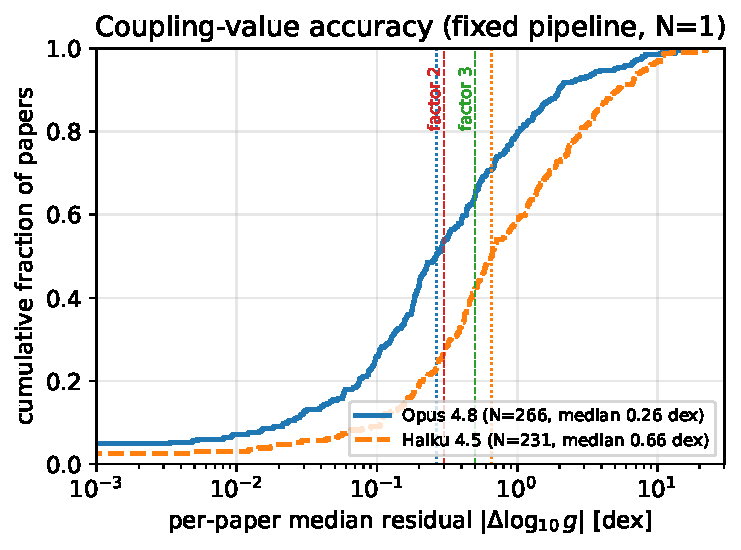
\includegraphics[width=0.52\textwidth]{figures/residual_cdf.pdf}
\caption{Cumulative distribution of per-paper median residuals for both arms
of the definitive benchmark. The model-tier gap is visible as a rightward
shift; the small model's heavier tail is the operationally relevant
difference.}
\label{fig:cdf}
\end{figure}

\begin{figure}[t]
\centering
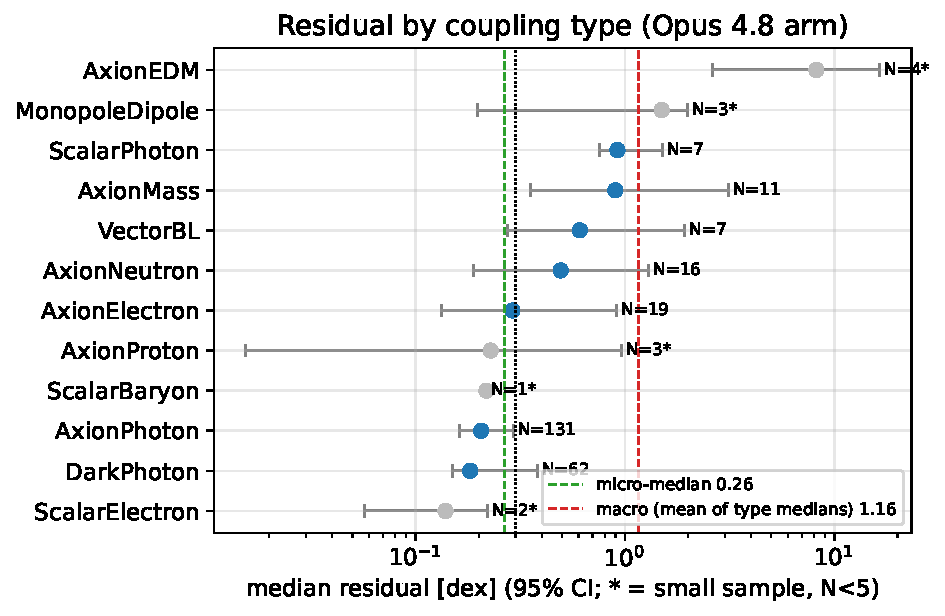
\includegraphics[width=0.52\textwidth]{figures/per_type_residual.pdf}
\caption{Median residual by coupling type with bootstrap 95\% CIs (production
arm). The micro--macro gap is concentrated in rare, convention-heavy types;
small-sample types ($N<5$) are greyed.}
\label{fig:pertype}
\end{figure}

\subsection{Where the difficulty now lives}
The micro--macro gap (0.2509 vs 0.629~dex) localises the remaining hard
problem (figure~\ref{fig:pertype}): rare coupling types with idiosyncratic
conventions---AxionEDM, monopole--dipole couplings, and small-$N$ scalar
types. AxionEDM illustrates both failure routes. Papers reporting the
oscillating-EDM response in e$\cdot$cm are deliberately \emph{excluded} as
convention gaps: mapping that response back to the operator coupling folds
in the assumed local dark-matter density and per-analysis numerical factors
with no closed form, so the registry cannot vet a constant conversion and
fails closed. Those exclusions, however, contribute nothing to the macro
tail --- the AxionEDM residuals come from papers that \emph{were} compared
and failed conventionally: mis-declared conventions and extractor arithmetic
slips that the registry accepted at face value. These types are also
misclassified most often, which removes them from the comparable pool
entirely and compounds their difficulty. Improvement here is per-coupling
registry and classification work, not further gains on the
AxionPhoton-dominated headline.

\subsection{Cost and calibration}
\label{sec:calib}
At production volume the model-tier price argument inverts: the small model is
$\sim$5$\times$ cheaper per extraction, decisive for bulk evaluation
(hundreds of papers), but at 1--3 papers/day the absolute difference is cents
per day while its 18\% catastrophic rate lands on the human reviewer's desk.
Production therefore runs the frontier model; benchmarks run the small one.
Confidence calibration on the production arm (figure~\ref{fig:calib}):
accuracy (residual $<0.32$~dex and coverage $\geq$50\%) rises monotonically
across the upper three of the four populated bins---33.3\%, 32.6\%, 48.5\%,
72.0\%---but the top bin remains overconfident (mean confidence 0.840
vs 0.720 accuracy). Confidence \emph{ranks} extractions usefully for review
triage; it cannot replace review. (An earlier version of this analysis
reported a $+0.69$ top-bin gap; that was primarily a scoring artefact---
correct extractions graded as failures by convention gaps---and the repaired
scoring is what we report.)

\begin{figure}[t]
\centering
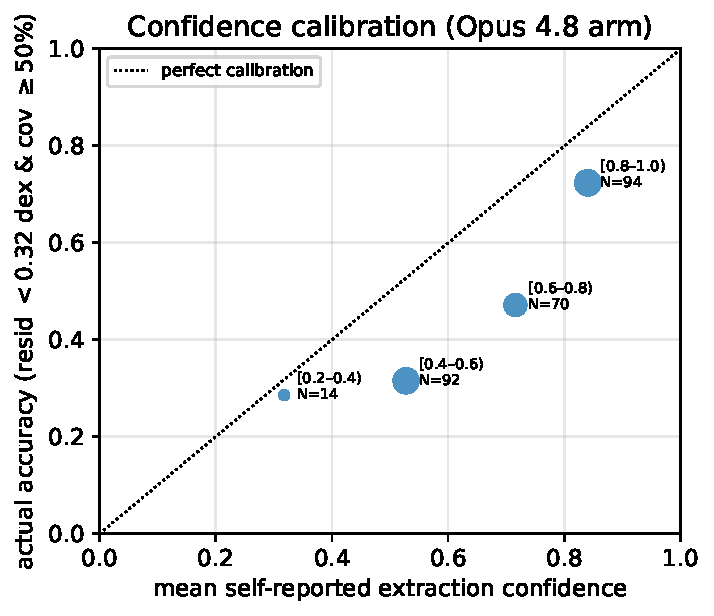
\includegraphics[width=0.52\textwidth]{figures/confidence_calibration.pdf}
\caption{Confidence calibration on the production arm. Marker area is
proportional to the number of papers in the bin. Accuracy is monotone in
confidence---a genuine ranking signal---but bins sit below the diagonal:
confidence triages review, it does not replace it.}
\label{fig:calib}
\end{figure}

\subsection{Case study: an end-to-end proposal on the release configuration}
\label{sec:cases}
To show the deployed behaviour end-to-end, we re-ran a paper through the
release configuration (frontier model, $N=1$) exactly as the daily pipeline
runs it, and present the proposal as its reviewer sees it. The paper --- the
QUALIPHIDE wideband dark-photon search~\cite{qualiphide}, whose limit is
already curated in the repository --- makes the resulting pull request a
direct pipeline-vs-curator comparison: the proposal's diff replaces the
curator's hand-digitised curve with the machine extraction. The audit trail:

\begin{itemize}
\item \emph{Pre-classification:} DarkPhoton, confidence 0.99.
\item \emph{Stage-2a axis identification:} $x\in[1, 40]$~$\mu$eV,
  $y\in[10^{-15},10^{-7}]$, declared plotted quantity ``kinetic mixing
  parameter $\chi$, dimensionless, log axis'' --- already canonical, so the
  registry applied no conversion (truthful-declaration path).
\item \emph{Validity-first selection:} the \emph{text} channel won over the
  figure-vision trace --- the paper states its bound in prose, and a stated
  bound outranks a trace of equal validity on the tier order
  (table~\ref{tab:channels}).
\item \emph{Density convention (single-owner):} the paper assumes local dark
  matter density $\rho=0.3$~GeV/cm$^3$ against the repository's
  0.45~GeV/cm$^3$. A haloscope limit scales as $\chi\propto1/\sqrt{\rho}$, so
  the repository stores each such limit paper-native and its \emph{single}
  plotting method applies the display rescale
  $\sqrt{\rho_{\rm paper}/\rho_{\rm repo}}=\sqrt{0.3/0.45}=0.816$ (a higher
  assumed density gives a stronger limit). The pipeline therefore stores the
  extraction paper-native and does \emph{not} duplicate the conversion --- the
  single-owner-conversion principle, here with the owner being the plotting
  method rather than the registry.
\item \emph{Result:} $\chi \lesssim 1.0\times10^{-12}$ over 19.7--30.5~$\mu$eV
  (extraction confidence 0.70), stored paper-native alongside the curator's
  own digitised curve ($\chi \approx 1.1$--$1.7\times10^{-12}$ over the same
  band at the same $\rho=0.3$). At matched density the two are directly
  comparable; the modest offset reflects the paper stating a single flat
  bound where the curator digitised a shallow curve, not a convention gap.
\item \emph{Integration:} because the experiment is already curated, the
  pipeline takes the update path (data-file replacement, no code change) and
  emits the highlighted plot of figure~\ref{fig:showcase}, bundled into a pull
  request for expert review.
\end{itemize}

\begin{figure}[t]
\centering
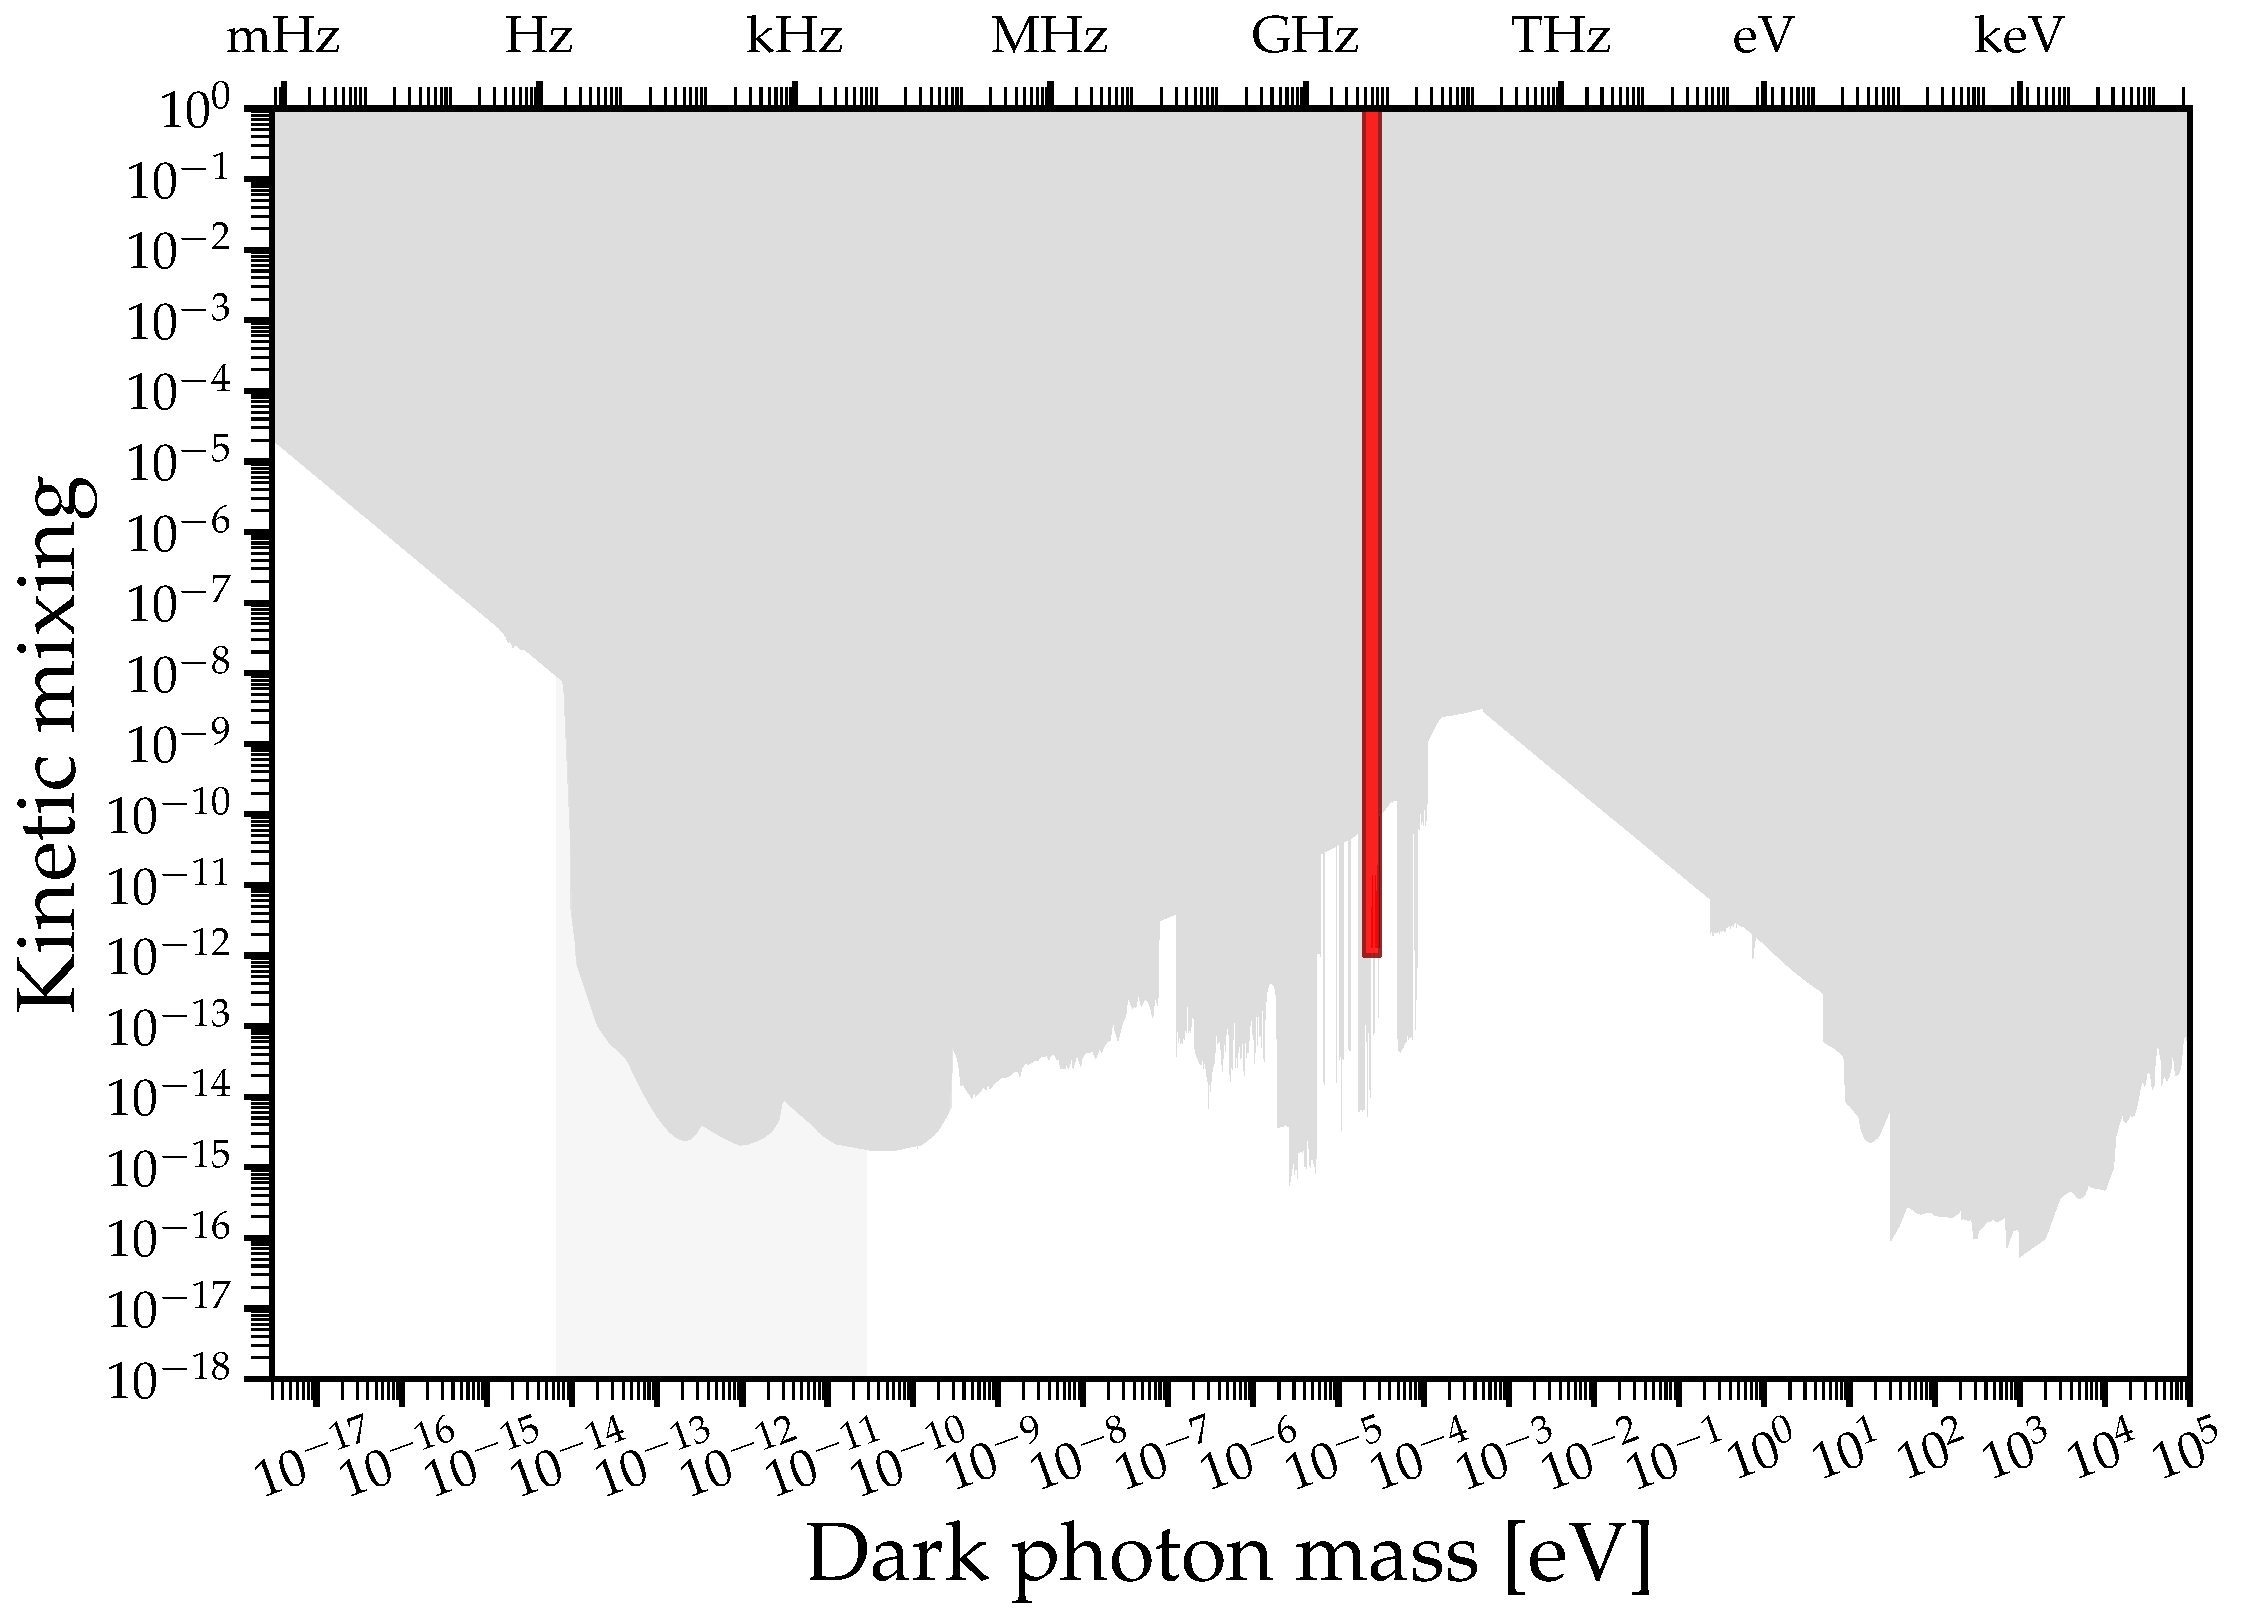
\includegraphics[width=0.72\textwidth]{figures/DarkPhoton_2209_03419_highlighted.pdf}
\caption{The reviewer-facing highlighted plot produced by the case-study
run: the full dark-photon compilation greyed out, with only the proposed
QUALIPHIDE update~\cite{qualiphide} in red (19.7--30.5~$\mu$eV,
$\chi\sim1.0\times10^{-12}$). A reviewer can judge the proposal's
plausibility in seconds without reading code.}
\label{fig:showcase}
\end{figure}

The same run was also instructive about the review gate's scope. Re-extracting
an already-curated experiment initially triggered an integration fault (a
name collision with the existing plotting method); it surfaced --- and was
fixed --- precisely because every output is a reviewable pull request rather
than an automatic merge. We note honestly what the gate does \emph{not} catch
on its own: the density-direction error discussed above was a deterministic
code fault that an expert reviewing the plotted curve would not necessarily
spot, and it was caught instead by independent scrutiny of this manuscript.
The lesson we draw is section~\ref{sec:discussion}'s: deterministic transforms
must be unit-tested at the source, because neither the model nor the visual
review gate is a reliable backstop for a sign error in arithmetic.

\paragraph{Operations.} The pipeline has operated on the live arXiv feed
since spring 2026 through the daily and weekly workflows described in
section~\ref{sec:arch}, with the historical backfill covering older
literature. Every proposal is opened as a pull request against our fork and
awaits expert disposition there; deliberately, no machine-generated limit
has been merged into the upstream community compilation --- the review and
governance mechanisms of section~\ref{sec:limitations} are, in our view, a
precondition, and the human gate is the point of the design rather than a
temporary scaffold.

%=============================================================================
\section{Lessons learned}
\label{sec:discussion}
%=============================================================================

\subsection{What helped}
Each of the following carries measured evidence from
sections~\ref{sec:results}.
\emph{Validity-first selection} over point-count routing (a quoted bound
cannot lose to a hallucinated trace on volume alone).
\emph{Deterministic channels wherever determinism is available}:
source-data harvesting and vector-path tracing are exact or near-exact
(table~\ref{tab:channels_result}) at negligible model cost.
\emph{Deterministic guards over prompt exhortations}: pure-function gates on
the model's own outputs fired 39 times in one benchmark run; a prompt asking
the model to ``be careful'' fires never.
\emph{Single-owner conversions with truthful-declaration and plotted-values
contracts}: the 8-dex anatomy (section~\ref{sec:anatomy}) is the argument.
\emph{Fail-closed escalation on unknown conventions}: 20 papers routed to
human review beats 20 silently wrong decades.
\emph{Cross-channel numeric corroboration}: an independent text anchor is the
cheapest available check on a vision trace.
\emph{The human-in-the-loop PR gate} as the safety backstop for everything
above.
\emph{Availability fail-fast and runtime configuration assertion}
(section~\ref{sec:ops}).
\emph{Confound-controlled evaluation with a measured noise floor}
(section~\ref{sec:confound}).
\emph{Prompt caching} (20--36\% of token spend).

\subsection{What did not help}
Equally valuable, with the evidence:
\emph{Consensus voting on a strong model}: $+0.003$~dex for $3\times$ cost
(section~\ref{sec:votes}); it stabilises the wrong variable.
\emph{Asking the model to convert units}: ``helpful conversion'' is poison---
it manufactures double or zero conversion downstream
(section~\ref{sec:anatomy}).
\emph{Substring matching of free-text convention declarations}: false
convertibles silently suppress review flags; match against the vetted
vocabulary instead.
\emph{Message-batch transport for heterogeneous agentic loops}: large vision
payloads serialise behind a single dispatcher; fine for homogeneous
small-payload jobs, a wedge for this one.
\emph{Trusting environment configuration without runtime assertion}: the
silent-model incident (section~\ref{sec:confound}) cost a full benchmark
cycle.
\emph{Single-run benchmark deltas below the noise floor}: 0.02--0.07~dex of
any single-run comparison is routing noise.

\subsection{Cross-cutting principles}
Keep the LLM to perception and semantics; keep arithmetic, unit conversion,
and selection deterministic and testable. Make every model claim
auditable---declarations, notes, and gate flags are what the guards, the
selector, and ultimately the human reviewer consume. Measure the noise floor
before claiming improvements. And treat evaluation methodology as part of the
instrument: the confound we caught (section~\ref{sec:confound}) would have
shipped a wrong conclusion about a $5\times$ cost decision.

%=============================================================================
\section{Limitations and future work}
\label{sec:limitations}
%=============================================================================
\emph{Channel-routing stability.} The residual run-to-run variance is
dominated by which channel wins, not what a channel reads; corroboration
mitigates but does not remove it. \emph{Figure perception.} Deterministic
vector-path tracing already covers the text-calibratable vector figures
(roughly a third of the corpus); the remaining raster and outlined-vector-text
figures are the irreducible perception floor, and reading them accurately
needs a pixel-geometry tracer or a specialist chart-extraction model inside
the validate-or-revert contract. Multi-curve figures additionally defeat curve
\emph{selection}---vision traces a projection, a compilation envelope, or a
neighbouring coupling's curve instead of the paper's own---which explicit
target-curve cues aim to fix before a specialist model is warranted.
\emph{Mass-window coverage.} Some extracted curves miss or overshoot the
ground-truth mass range; a wrong-window gate rejects the catastrophic
($\geq$3~dex) cases, but finer drift tolerance, using the figure's own axis
range as a second window source, and auto-correcting constant-factor mass-axis
unit offsets ($\mu$eV$\leftrightarrow$eV, GHz$\leftrightarrow$eV) would
\emph{recover} such curves rather than reject them. \emph{Coupling-type
classification.} The residual $\sim$8\% of misclassifications concentrate in
rare, confusable types (vector $B\!-\!L$ vs.\ dark photon, scalar sub-types,
AxionMass/EDM/CPV), each a \texttt{no\_comparable\_gt} double penalty and a
driver of the micro--macro gap; targeted disambiguation cues and
vote-agreement escalation are the path. \emph{Text-anchor generalisation.} The
corroboration gate needs an in-range text anchor; abstract-stated bounds could
widen its coverage. \emph{Registry growth.} Unknown conventions currently stop at the
review flag; the planned loop drains them offline---queued, expert-vetted
(with LLM assistance), then released to the registry---so the vetted
vocabulary grows without ever guessing at runtime. \emph{Distributional
benchmarks.} Given the noise floor, 2--3 repeat runs per configuration would
turn single-run point estimates into distributions. \emph{Per-stage model
tiering.} Pre-classification does not need a frontier model; tracing might.
\emph{Upstream adoption and governance.} The pipeline proposes; the curator
community disposes. Reviewing machine-proposed limits at scale needs a
process---a community editorial board analogous to the Particle Data Group
reviewers~\cite{pdg}, where collaborations validate their own limits, is one
model. More fundamentally, the infrastructure for machine-readable limit
publication is already established and in routine use: HEPData~\cite{hepdata}
archives digitised collider results as standard practice, and the LHC Reinterpretation
Forum has published community recommendations for reusable result
presentation~\cite{reinterpretation_forum}. The gap is not tooling but
\emph{adoption in the ultralight-dark-matter community}, where results are
still published predominantly as figures. Extending the HEPData habit to
this subfield would bypass the extraction problem this paper mitigates, and
remains the single highest-leverage change available; until then, extraction
pipelines like this one are the bridge.

%=============================================================================
\section{Conclusions}
\label{sec:conclusion}
%=============================================================================
An LLM-agent pipeline with deterministic guards curates the live dark matter
limit literature at a median accuracy of 0.25~dex among compared
measured-limit papers---within a factor of two at over half the measured
points---with a $\sim$6\% catastrophic rate among compared papers, at one
LLM read per paper, with every output reviewed by a human
before anything merges. The measured decomposition is the point: the decisive
engineering was not the model but the architecture around it---deterministic
channels and guards, single-owner convention canonicalization with
fail-closed escalation, and confound-controlled measurement with a known
noise floor. The frontier model earns its place in the tail (a roughly $3\times$ lower
catastrophic rate), not the median ($+0.21$~dex);
consensus voting earns no place at all. We offer the pipeline, the benchmark, and these measured
lessons to the community whose infrastructure problem motivated them.

%=============================================================================
\acknowledgments
%=============================================================================
We acknowledge funding support from Dianzhuo Wang and TwentyTwo.

\paragraph{AI-use declaration.}
Large language models are both the subject of and a tool in this work, and we
declare their use in detail. The extraction and review agents of the pipeline
itself run Anthropic Claude models: \texttt{claude-opus-4-8} in the production
configuration and \texttt{claude-haiku-4-5} in the evaluation arm, as
benchmarked in section~\ref{sec:results}. The pipeline's code and this
manuscript were developed with the assistance of Claude models (including
Claude Code agents) under human direction; all conversion factors in the
convention registry were derived and citation-audited with the GPD
assistant~\cite{gpd} and code-verified by the authors. Every number in
section~\ref{sec:results} is generated by committed scripts from committed
benchmark artifacts. All scientific claims, numerical results, and the final
text were verified and approved by the authors, who take full responsibility
for the content.

%=============================================================================
\section*{Data and software availability}
%=============================================================================
The pipeline source code, the evaluation benchmark, the scoring
code, the extraction prompts, the benchmark artifacts
(\texttt{evaluation/eval\_runs/final2\_*}), and the scripts in
\texttt{paper/} that generate every number and figure in this paper
(\texttt{make\_paper\_numbers.py}, \texttt{make\_journal\_figures.py}) are
openly available at \url{https://github.com/FaroutYLq/AutoAxionLimits}. A versioned archive with
a persistent DOI will be deposited at submission. % TODO: mint Zenodo DOI before submission.
The upstream constraint data are from the AxionLimits
repository~\cite{axionlimits}.

\bibliographystyle{JHEP}
\bibliography{refs}

\end{document}
